\section{Convex Optimization Problem Classes}

\subsection{Feasibility Problems}
Reduce to checking whether the optimal value of an auxiliary problem
with slack \(s\) is non-positive.

\subsection{Linear Programming (LP)}
\[
  \min c^\top x\quad\text{s.t.}\quad Ax-b\ge 0,\;x\ge 0.
\]
Its dual is again an LP. Optimal solutions, when they exist, lie at
vertices of the polyhedron.

\subsection{Quadratic Programming (QP)}
\[
  \min\tfrac12 x^\top Px+q^\top x\quad\text{s.t.}\quad Gx\le h,\;Ax=b.
\]
Convex when \(P\succeq 0\).

\subsection{Second-Order Cone Programming (SOCP)}
\[
  \min f^\top x\quad\text{s.t.}\quad \|A_ix+b_i\|\le c_i^\top x+d_i.
\]
The second-order cone \(C_{n+1}=\{(x,t):\|x\|\le t\}\) is self-dual
and admits efficient projection.

\subsection{Semidefinite Programming (SDP)}
\[
  \min\langle C,X\rangle\quad\text{s.t.}\quad\langle
  F_i,X\rangle=b_i,\;X\succeq 0.
\]
SDP is the most general convex problem class that can still be solved
in polynomial time (to any fixed accuracy) by interior-point methods.

\textbf{Hierarchy of problem classes.} LP \(\subset\) QP \(\subset\)
SOCP \(\subset\) SDP.

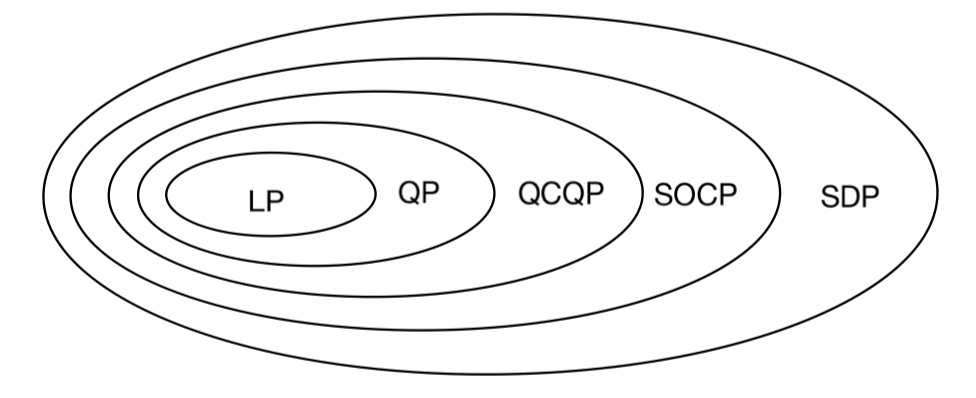
\includegraphics[width=\columnwidth]{images/problem_class.png}

